% Based on Model 1 of Activity 5 - Strings by Helen Hu

\model{Character Arrays}

The primitive type \java{char} is used to store a single character, which can be a letter, a number, or a symbol.
In contrast, the reference type \java{String} \emph{encapsulates} an array of characters.

\begin{minipage}[t]{150pt}
\begin{javalst}
char letter;
letter = 'A';

char[] array;
array = new char[]
        {'c', 'a', 't'};

String word;
word = "dog";
\end{javalst}
\end{minipage}
\hfill
\begin{minipage}[t]{345pt}
\null
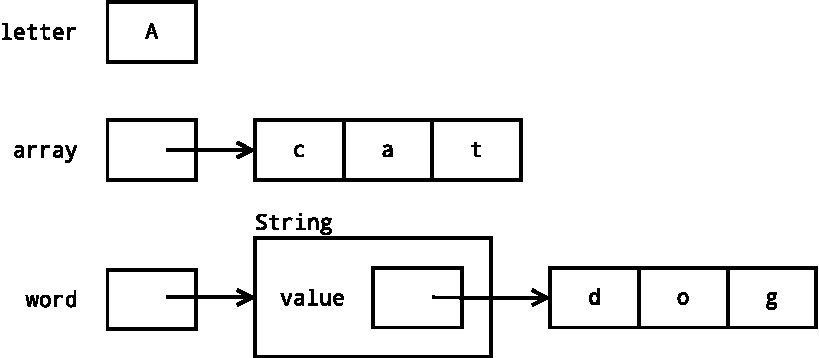
\includegraphics[width=\linewidth]{string1.pdf}
\null
\end{minipage}


\quest{15 min}


\Q How is the syntax of character literals and string literals different?

\begin{answer}
Character literals use single quotes, and strings use double quotes.
\end{answer}


\Q What is the index of \java{'d'} in the string above?
What is the index of \java{'g'}?
In general, what is the index of the last character of a string?

\begin{answer}
The index of \chr{d} is 0, the index of \chr{g} is 2.
In general, the last character is at {\tt length - 1}.
\end{answer}


\Q Based on the diagram, what does it mean for a class to encapsulate data?
How do you access data inside of a class?

\begin{answer}
The data is stored inside the class and accessed via methods.
\java{String} (the class) makes it more convenient to deal with character arrays.
\end{answer}


\Q Why can you use the \java{String} class in Java programs without having to import it first?

\begin{answer}
It's in the \java{java.lang} package, which gets imported automatically.
\end{answer}


\Q What is the value of a \java{char} variable?
What is the value of an array variable?
What is the value of a \java{String} variable?

\begin{answer}
Since {\tt char}s are primitive, the value of a {\tt char} variable is the character itself.
Arrays and strings are reference types, so their variables contain memory locations.
\end{answer}


\Q Draw a memory diagram for the given code.
Each variable should be a name next to a box containing its value.

\vspace{1ex}
\begin{javalst}
String str;
str = "Hi!";

char let;
let = 'X';

int num;
num = -1;

double foo;
foo = num;

String hmm;
hmm = str;
\end{javalst}

\vspace{-3.25in}
\begin{answer}[3.1in]
\hspace{2.2in}
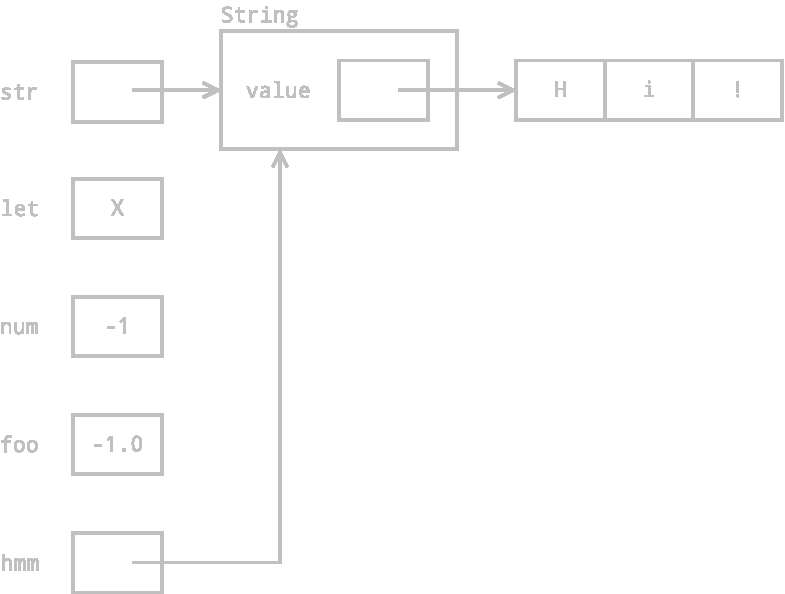
\includegraphics[height=3in]{string2.pdf}
\end{answer}


\Q Recall that the \java{==} operator compares the \emph{value} of two variables.
What does it mean for two \java{char} variables to be \java{==}?
What does it mean for two \java{String} variables to be \java{==}?

\begin{answer}
Two {\tt char} variables are \java{==} if they have the same character.
In contrast, two {\tt String} variables are \java{==} if they refer to the same \java{String} object.
\end{answer}


\Q How could you determine whether two character arrays have the same contents?
In other words, how does the \java{Arrays.equals} method work internally?

\begin{answer}
Using a loop, you compare each character in the first array to the corresponding character in the second array. If any two characters don't match, or the arrays have different lengths, then they are not equal.
\end{answer}
